
\chapter{Introducción}

La piel es considerada el órgano más grande del cuerpo humano; está compuesta por tres capas: \emph{\gls{epidermis}}, \emph{\gls{dermis}} e \emph{\gls{hipodermis}} (figura \ref{fig:skin1_jpg}). La principal función de la piel es proteger al cuerpo de las hostilidades del medio ambiente como la radiación solar y los factores externos como las bacterias, sin embargo también cumple otras funciones importantes aparte de proteger los órganos y los tejidos internos, tales otras funciones son regular nuestra temperatura corporal, registrar sensaciones de presión, frío, calor y es una interfaz para poder sentir e interactuar con lo que tenemos a nuestro alrededor.

\begin{figure}[h!]
    \includegraphics[width=80mm, scale = 0.5]{Figuras/skin_structure_esp.eps}
    \centering
    \caption{Ilustración de las capas de la piel y sus apéndices \citep{skin_1}.}
    \label{fig:skin1_jpg}
\end{figure}

Sin embargo, debido a la exposición continua a las radiaciones de la luz es común desarrollar enfermedades en la piel que afectan la forma en que las células de la piel se reproducen, causando graves daños en el tejido celular y en algunos casos resultando letal. Estas anomalías en la piel se denominan como \emph{cáncer de piel}, y se clasifican de la siguiente forma: cáncer de células basales, cáncer de células escamosas y melanomas \citep{cancer_org}.

\begin{figure}[h!]
    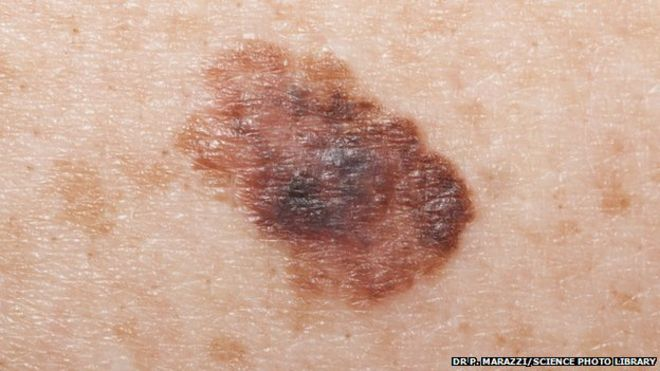
\includegraphics[width=80mm]{Figuras/skin_cancer_bbc.jpg}
    \centering
    \caption{Ejemplo de melanoma \citep{cancer_img_1}.}
    \label{fig:can_jpg}
\end{figure}

 Su detección temprana es imprescindible para reducir las probabilidades de fallecimiento. Por lo tanto es necesario seguir desarrollando tecnologías que faciliten la detección de este tipo de padecimientos de forma rápida y sencilla; y que vaya enfocada en aumentar la accesibilidad a dichos diagnósticos y de esta forma reducir la tasa de mortalidad por este padecimiento.

En los últimos años se han logrado muchos avances en cuanto al desarrollo de software inteligente lo cuál ha permitido un mayor acceso a diferentes servicios, una de las tecnologías que han adquirido mayor importancia es la \emph{\gls{rn}}, se trata de una tecnología que tiene la capacidad de \emph{aprender} mediante el úso de datos históricos y mediante funciones de optimización crear un modelo matemático capaz de predecir, clasificar o recrear datos futuros o desconocidos. Algunos de los sectores que han comenzado a adoptar esta tecnología son: el sector automotriz (piloto automático), el sector de manufactura (optimización de procesos), el sector de entretenimiento (recomendaciones personalizadas), el sector médico (diagnóstico de imágenes). 


\section{Hipótesis}
Es posible clasificar los píxeles en distintas categorías dentro de una imagen gracias a las avances actuales de inteligencia artificial y la técnica de segmentación. Mediante la técnica de \emph{\gls{seg}} es posible crear un reconocedor visual que no solo detecte la presencia y ubicación del elemento a reconocer, sino que, también obtenga otros datos descriptivos del elemento como el tamaño, forma y región que abarca dentro de la imagen.

\section{Objetivos}
Primero en \emph{objetivo general} se habla de manera conceptual la problemática a resolver tales como cuales son las situaciones en las que podemos optimizar la resolución de un problema mediante el uso de la red neuronal, posteriormente en los \emph{objetivos específicos} se describe de forma puntual los pasos a realizar en el presente trabajo de tésis para llegar al resultado deseado.

El \emph{objetivo general} de este trabajo de tésis es la creación de una aplicación con la capacidad de reconocer y segmentar melanoma en la piel de forma automatizada, con el motivo de asistir a los médicos dedicados a esta labor a optimizar y extender la detección temprana, consiguiendo así una reducción en su mortalidad.

El \emph{objetivo específico}, es el implementar un modelo de red neuronal cuya entrada sean imágenes que pueden o no contener la presencia de alguno de los tipos de cáncer de piel comunes, y como salida del modelo se obtenga un mapa de características donde de haber presencia de el cáncer este se distinga mediante una región colorada en el espacio que abarca. El modelo debe cumplir con las siguientes características:

\begin{itemize}
    \item El modelo debe ser capaz de trabajar con imágenes a color o en blanco y negro.
    \item El modelo debe contar con una función capaz de evaluar la precisión.
    \item El modelo debe contar con un algoritmo capaz de optimizar la precisión.
    \item El modelo debe ser capaz de segmentar correctamente imágenes no usadas en los datos de entrenamiento.
\end{itemize}

\begin{figure}[!htp]
    \centering
    \subfloat[imágen real de entrada]{\label{a_1}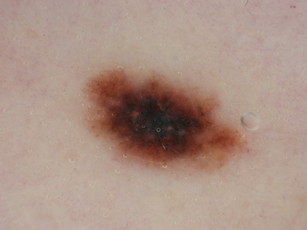
\includegraphics[width=50mm]{Figuras/input_1.png}}
    \qquad
    \subfloat[máscara de salida]{\label{b_1}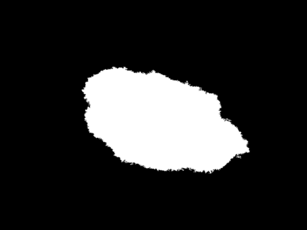
\includegraphics[width=50mm]{Figuras/mask_1.png}}
    \caption{Ejemplo de segmentación: entrada y salida.}
    \label{data_1}
\end{figure}

En la figura \ref{a_1} se observa como la imagen entrante presenta un caso de melanoma, mientras que la figura \ref{b_1} se puede observar la misma imagen después de pasar por una secuencia de transformaciones, esto se denomina \emph{segmentación semántica} y se refiere a la acción de separar y clasificar en una o más categorías los objetos detectables en una imagen.

\section{Estructura de la Tesis}
A continuación se da una breve explicación sobre el orden en el que se presentan los capítulos de este trabajo de tesis, así como una breve descripción de su contenido.

En el capítulo 2 se habla sobre los antecedentes relacionados al presente trabajo de tesis, primero se empieza definiendo la naturaleza del problema con el que se pretende tratar, después algúnos conceptos clave que serán necesarios para la comprensión de la implementación propuesta tales como las dimensiones de los datos y los algoritmos de evaluación y optimización.

En el capítulo 3 se recopilan trabajos relacionados al método o problemática en cuestión, se estudia las características de dichos trabajos y se busca un punto de convergencia entre estos y el presente trabajo de tésis con el fin de comparar las áreas de oportunidad.

En el capítulo 4 se define el proceso de transformación de los datos del sistema propuesto en este trabajo de tesis, desde las características de los datos a la entrada.

El capítulo 5 describe a profundidad la implementación de la propuesta, desde la descripción de los datos utilizados para el entrenamiento del modelo y la verificación de este, la arquitectura específica utilizada 


Finalmente, en el capítulo 6 se exponen los resultados obtenidos de la implementación del producto científico en el capítulo anterior, así como un análisis y conclusión final sobre los valores obtenidos en precision y tiempo de entrenamiento. 

\chapter{Antecedentes}
En este capítulo se introduce de forma teórica conceptos relacionados con el trabajo propuesto, primero se define que es el \emph{cáncer de piel}, cuales son los factores que influyen en el desarollo de este padecimiento, los tipos de cáncer y las diferencias entre estos. Después algunos conceptos relacionados con las redes neuronales necesarios para un entendimiento sólido del \emph{aprendizaje profundo}, tales como los elementos clave que conforman a la red neuronal, la manera en la que esta evalúa su precisión, y el algoritmo de optimización.

\section{Cáncer de Piel}
El \emph{cáncer de piel} es una enfermedad que suele relacionarse con la aparición de lunares o manchas que no se encontraban previamente, se pueden manifestar como manchas oscuras o rojizas, bultos y/o escamas en la superficie de la piel y afecta a todos los tonos de la piel por igual. Esta enfermedad se desarrolla principalmente en partes del cuerpo expuestas al sol, sin embargo también se puede desarrollar en partes que no suelen exponerse. Algunos factores como la exposición a los rayos ultravioletas (UV), el uso de sustancias como el tabaco o el envejecimiento son factores correlacionados con la aparición del \emph{cáncer de piel}, existen dos factores de envejecimiento y se dividen en dos grupos: \emph{intrínsecos} y \emph{extrínsecos}.

Los factores \emph{intrínsecos} son aquellos que suceden de forma interna en la piel, un ejemplo de esto es el envejecimiento cronológico, el cual es un proceso natural que consiste en degradación del colágeno, la elastina y el adelgazamiento de la epidermis debido al envejecimiento celular al paso de los años y de el efecto de algunas hormonas.

Los factores \emph{extrínsecos} son aquellos que suceden de forma agena al organismo, como es el caso del \emph{foto-envejecimiento} el cual sucede cuando nos encontramos expuestos a los rayos ultravioletas (UV). Este factor de envejecimiento genera lesiones en las cadenas de ácido desoxirribonucleico (ADN) debido a la oxidación y afecta la regeneración de celulas, al sistema inmune y a la forma en la que se regula la pigmentación \citep{skin_aging}.

\subsection{Tipos de Cáncer de Piel}
El cáncer de piel es un padecimiento que se puede manifestar en una gran variedad de formas distintas, algúnas de estas formas pueden representar un enorme riesgo para la salud de quien la padece mientras que otras pueden permanecer mucho tiempo sin afectar la calidad de vida del paciente; se clasifican principalmente en dos tipos: \emph{benigno} y \emph{maligno}.

Los tumores del tipo \emph{benignos} no suelen ser considerados cáncer como tal, ya que tienen un crecimiento lento y no suelen extenderse a otras partes del cuerpo, por otro lado los tumores \emph{malignos}, si representan un riesgo mayor ya que crecen rapidamente y suelen hacer \emph{metástasis}, osea que migran a otras partes del cuerpo. 

\section{Redes Neuronales}

Hasta hace algunos años el desarrollo de aplicaciones de software solía realizarse de forma robústa, por ejemplo, si deseáramos desarrollar una aplicación de reconocimiento de imágenes faciales de la forma tradicional, sería necesario un grupo de expertos en dicho rubro para que definan una secuencia de transformaciones específicas para lograr esa función, donde la variabilidad de las imágenes que dicho sistema permitiría depende específicamente de la complejidad del mismo, sin embargo mediante las redes neuronales es posible resolver el mismo problema con la ventaja de que la variabilidad de imágenes que pueden ser reconocidas por el sistema, depende de los datos utilizados para el entrenamiento, el model de una red neuronal \emph{aprende} de los datos proporcionados y crea un modelo capaz de clasificar, predecir o reconstruir datos conocidos y desconocidos. Algunos de los puntos clave que conforman un sistema basado en redes neuronales son:

\begin{description}
    \item[Datos]{Se debe determinar la naturaleza y la dimensión de los datos que entrarán al modelo.}
    \item[Modelo] {Se debe crear un sistema que transforme los datos de entrada, en la salida deseada.}
    \item[Evaluación] {El modelo debe tener la capacidad de evaluar su precisión.}
    \item[Optimización] {El modelo debe contar con un algoritmo que optimice la precisión.}
\end{description}

\subsection{Imágenes como Datos}
Las imágenes se pueden definir como una matriz de $m \times n \times 1$ pixeles en el caso de las imágenes de un solo canal (blanco y negro) y en el caso de imágenes a color es de $m \times n \times k$, donde $k$ es igual al numero de canales de color que tenga la imagen, siendo tres en el caso de imágenes RGB\footnote{RGB: Se refiere a los tres canales de color rojo, verde y azul, por sus siglas en inglés (\emph{red, green, blue}).}, es importante definir si las imágenes ingresarán al modelo a color o en blanco y negro debido a que esto define el numero de nodos de entrada de este, ya que para cada pixel debe corresponder un nodo de entrada y en el caso de imágenes a color también deberá tener un número de capas de nodos de entrada igual al número de canales que tenga la imagen.


\begin{figure}[!htp]
    \centering
    \subfloat[imagen de un solo canal]{\label{a}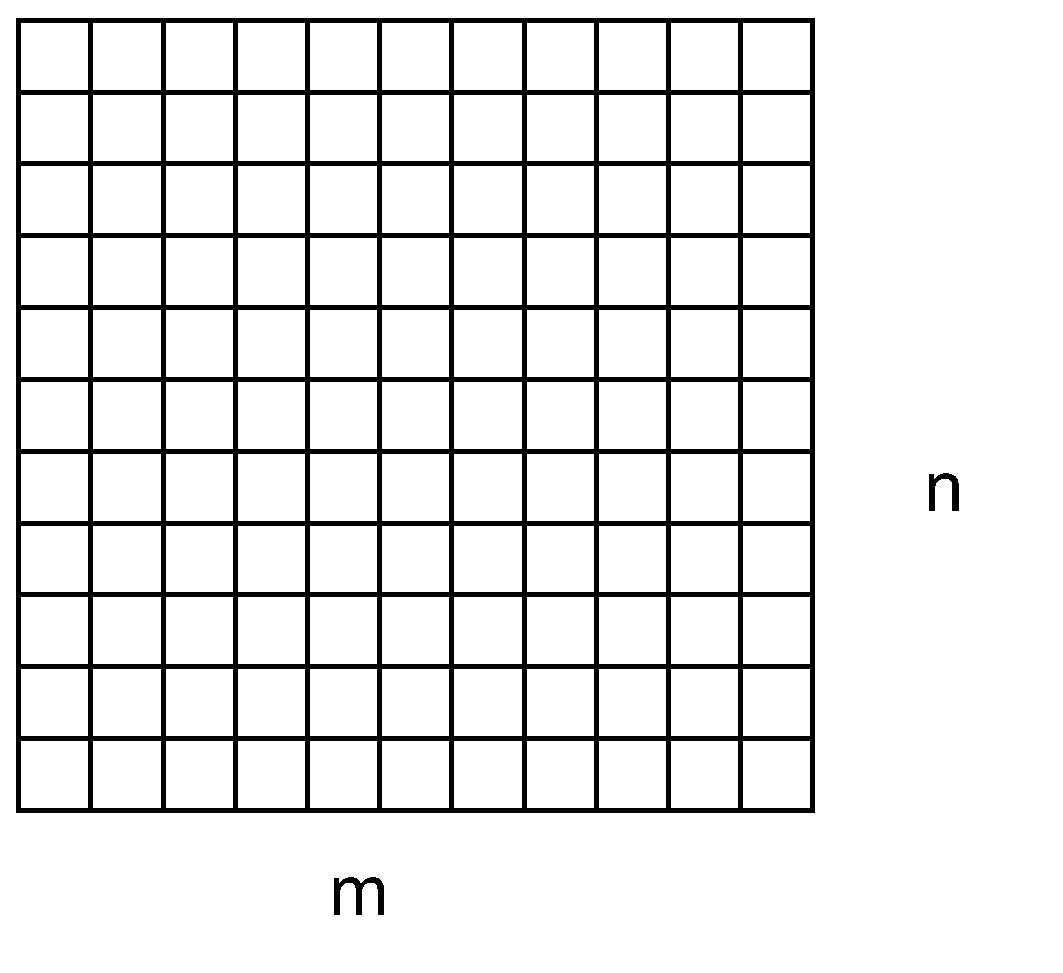
\includegraphics[width=50mm]{Figuras/bg_matrix.eps}}
    \qquad
    \subfloat[imagen de triple canal]{\label{b}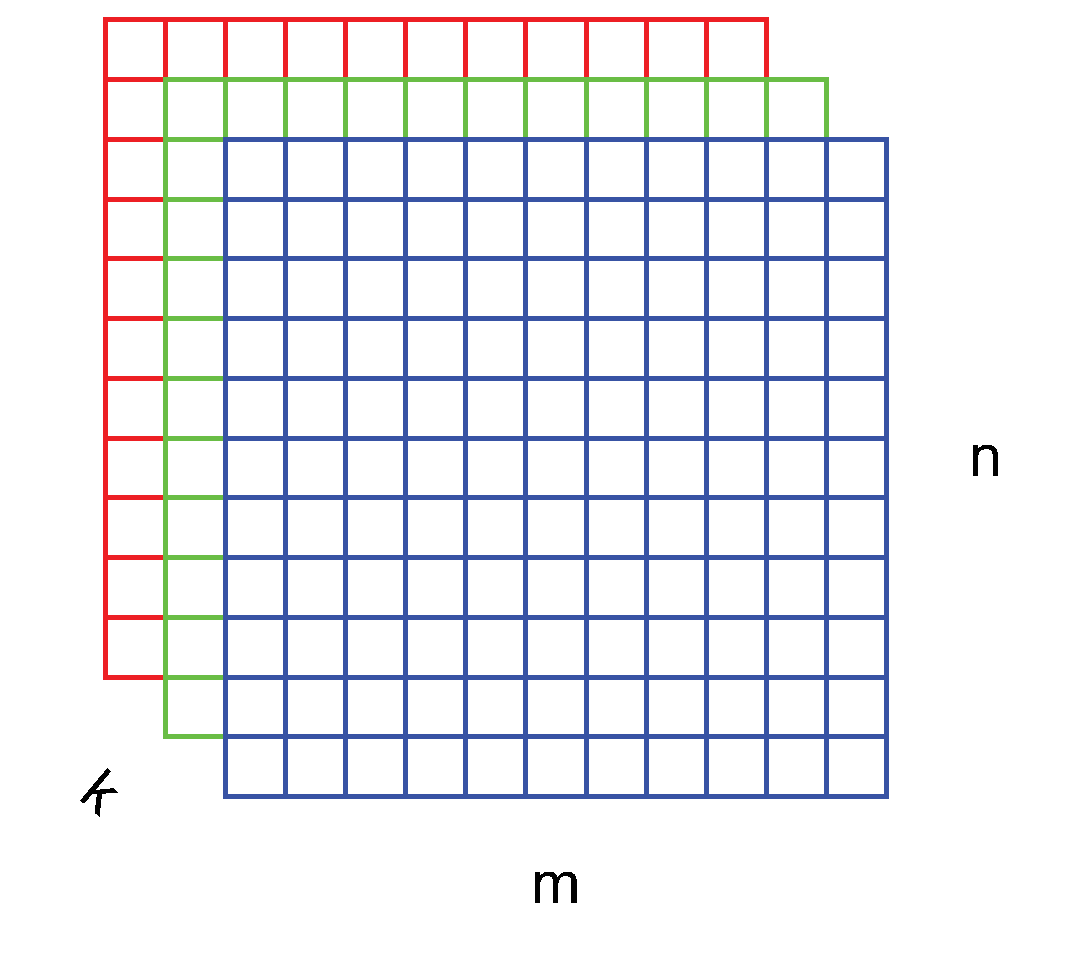
\includegraphics[width=50mm]{Figuras/rgb_matrix.eps}}
    \caption{Comparación de dimensiones en imágenes en blanco y negro e imágenes a color.}
\end{figure}

\subsection{Modelo}
Un \emph{modelo} se puede definir como el bloque intermedio entre los datos de entrada (\emph{input}) y los datos de salida (\emph{output}), es el sistema encargado de transformar los datos de entrada en la salida deseada y consta de los siguientes componentes:

La unidad principal que compone el modelo de la red neuronal es el perceptrón, denominado \emph{nodo} en esta literatura. Se trata de una analogía matemática basada en el comportamiento de la neurona biológica, el nodo recibe $n$ entradas, las cuales son multiplicadas por el peso $p$, se suma el producto de las entradas por sus pesos $ e \times p$ y finalmente se multiplica por la función de activación $\phi$. 

\begin{figure}[b]
    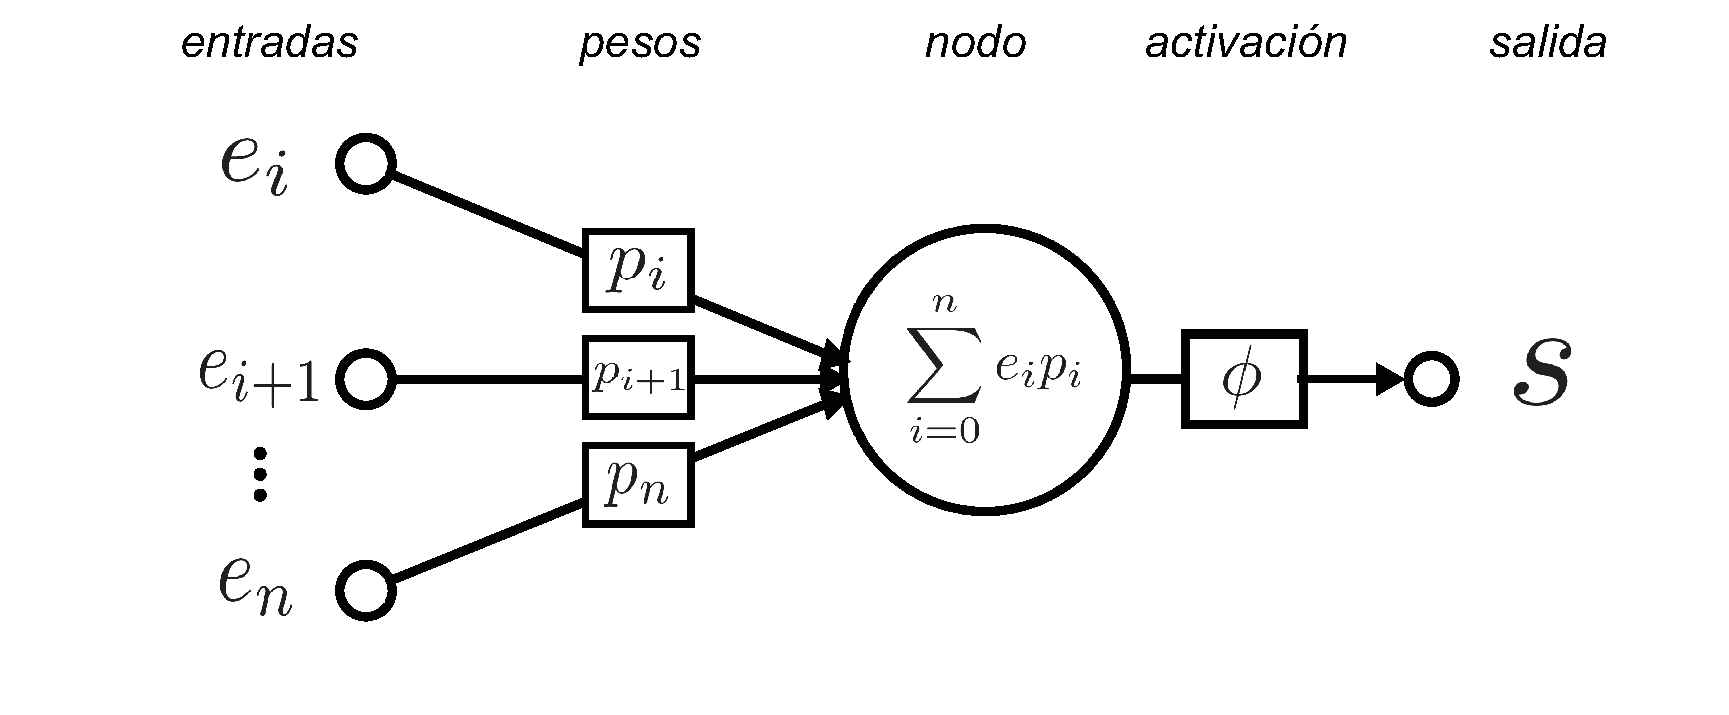
\includegraphics[width=100mm]{Figuras/neural_network.eps}
    \centering
    \caption{Ejemplo de un perceptrón.}
    \label{fig:percep}
\end{figure}

Partiendo de lo anterior, creando arreglos con estos nodos podemos formar estructuras denominadas \emph{redes neuronales}, las cuales cuentan con los siguientes elementos estructurales:

\begin{description}
    \item[Capa de entrada (\emph{input layers})] { Se trata de la primera capa del modelo, en el caso de imágenes a cada pixel le corresponde un nodo de entrada. Estos nodos deben tener las mismas dimensiones que las imágenes de entrada.}
    \item[Capa oculta (\emph{hidden layer})] {Las dimensiones de estos nodos pueden ser diferentes a los de entrada y tener varias capas ocultas, sin embargo esto puede afectar la complejidad y precisión del modelo.} 
    \item[Capa de salida (\emph{output layer})]  {Esta es la capa de salida del modelo, las dimensiones de la capa de salida determinan las dimensiones del dato resultante}
    \item[Función de activación (\emph{activation})]{Se trata de una función dentro de cada nodo que interactúa con el valor entrante y se multiplica por el peso.}
    \item[Pesos (\emph{weight})] {Se trata de un valor entre el nodo de la capa actual y el nodo siguiente inicializado de forma aleatoria y después ajustado por un algoritmo para aproximar la salida al valor real.}  
    \item[Sesgo (\emph{bias})] {Se trata de un valor constante que se suma al resultado de la función de activación y el peso, de esta forma se puede ajustar que tan fácil o difícil es activar un nodo.} 
\end{description}

\subsection{Evaluación y Optimización}
Para realizar el proceso de \emph{aprendizaje} del modelo, primero se debe evaluar cuál es el estado actual de las predicciones. Para esto es necesario evaluar que distancia existe entre el valor predicho y el valor real, esto se puede lograr mediante una \emph{función de pérdida} que se encargue de determinar que tanta diferencia (\emph{loss}) existe en las estimaciones del modelo con los pesos actuales.

Un ejemplo de la función de pérdida es el de la función logarítmica del costo (\emph{log-likelihood}), como se muestra a continuación

\begin{equation}
    l(\mathbf{y}, \hat{\mathbf{y}}) = - \sum_{j=1}^q y_j \log \hat{y}_j     
\end{equation}

$q$ representa el número de clases entre las cuales predecir, $y_j$ representa el valor de salida real, $\hat{y_j}$ el valor estimado de salida por el modelo y $j$ la posición indizada de clase.

Ya que se tiene calculada la pérdida del modelo en su configuración de pesos actual, es necesario actualizar el valor de todos los pesos dentro del modelo para poder acercarnos al valor real. Aquí es donde participa el algoritmo de \emph{gradiente descendiente} \citep{alg:gradient}, dicho algoritmo se puede representar con la siguiente ecuación

\begin{equation}
        Error = \frac{\partial}{\partial m} = \frac{2}{N}\sum_{i=1}^{N}-X_i(y_i-(mX_i+b))
\end{equation}

\begin{equation}
        \frac{\partial}{\partial b} = \frac{2}{N}\sum_{i=1}^{N}(y_i-(mX_i+b)) 
\end{equation}

donde $m$ y $b$ son valores enteros que representan el peso de dos parámetros de un modelo, los cuáles serán optimizados para acercar la salida del modelo a la salida real.

%\begin{algorithm}
%    \begin{algorithmic}
%        \For{$k = 0, 1 , 2 \dots n$}{
%
%            $g_k \leftarrow \nabla f(x_k)$ 
%           
%            $x_{k+1} \leftarrow x_k - t_k g_k$
%            }
%    \end{algorithmic}
%\end{algorithm}


\chapter{Estado del Arte}
En este capítulo se estudia las literaturas relacionadas con el presente trabajo de tesis con el objetivo de hacer una comparativa entre distintos métodos para resolver el mismo problema, o implementaciones similares para resolver problemas distintos.

En la primera sección, \emph{trabajos similares}, se recopilan trabajos con características relacionadas al presente trabajo de tesis, ya sea relacionados con el método o con el problema que se pretende resolver, se describe el tema que abarcan y los puntos que lo relacionan con el trabajo aquí presente.

En la segunda sección, \emph{análisis comparativo}, se comparan las distintas características de los trabajos revisados, de esta forma podemos determinar las principales diferencias así como las ventajas y desventajas de cada trabajo. Así mismo se recopilaran todas estas diferencias en una tabla para visualizar mejor estas características.

Finalmente en las \emph{áreas de oportunidad}, se realiza una conclusión acerca de los resultados en la tabla comparativa.

\section{Trabajos Similares}

A continuación se mencionan los trabajos revisados en los que se puede obtener un punto de convergencia ya sea en los métodos similares utilizados para resolver problemas diferentes o en su defecto métodos distintos para resolver problemas similares.

\citet{DBLP:journals/corr/BadrinarayananK15} en este trabajo se habla sobre la arquitectura denominada \texttt{SegNet} utilizada principalmente para la conducción autónoma y la detección de peatones, se describe como una arquitectura convolucional, con la característica de que es una jerarquía de codificador-decodificador donde a cada codificación (\emph{encoding}) corresponde una capa de agrupación de máximos (\emph{max pooling}) y un decodificador. Inspirado principalmente en la arquitectura \texttt{VGG16}, con la diferencia de que el componente clave en esta arquitectura es el uso de convoluciones en lugar de la capa completamente conectada de nodos (\emph{fully-connected-layer}) a la salida.

\citet{DBLP:journals/corr/RonnebergerFB15} proponen uno de los primeros modelos de la redes neuronales convolucionales denominada \texttt{U-net} dirigida al análisis de imágenes del area médica. Este trabajo consiste en una arquitectura con dos trayectorias: la trayectoria de contracción de la imagén y la trayectoria de expansión. En la trayectoria de contracción de la imagen se aplica una secuencia de convoluciones de dimension $3 \times 3$ con solapado, seguido de una función de activación de rectificación linear unitaria (ReLu) y posteriormente una operación de agrupación de máximos (\emph{max pooling}) para la compresión de la imagen (\emph{downsampling}). Por otro lado, la trayectoria de expansión consiste de el escalado de la imagen (\emph{upsampling}), en cada paso se aplica una capa de convolución de $2 \times 2$ a la cuál se concatena una imagen recortada del mapa de características de la trayectoria de contracción y dos convoluciones de $3 \times 3$ seguidos de una activación ReLu cada una. En total la arquitectura tiene 23 convoluciones (U-net).

\citet{DBLP:journals/corr/ChenPK0Y16} en este trabajo hablan de la arquitectura denominada \texttt{Deep Lab}, la cual propone un acercamiento distinto a la parte de la reconstrucción en las capas finales del modelo. Al igual que otras arquitecturas cuenta con capas de convolución. agrupación de máximos y activación de rectificación linear unitaria, sin embargo, el componente clave aquí es la denominada convolución de hoyos (\emph{atrous convolution}), la cual es una modificación al filtro de convolución basado en la transformada de \emph{Wavelet} para el escalado del mapa de características (\emph{upsampling}). De esta forma se obtiene una alternativa al uso de capas de deconvolución y así se aumenta la resolución del mapa de características a la salida del modelo sin aumentar el tiempo de computación o la cantidad de parámetros.

\citet{DBLP:journals/corr/TeichmannWZCU16} reducen la carga computacional en los modelos de redes neuronales convolucionales mediante la unificación de las tres tareas principales de estas: clasificación, detección y segmentación. Denominada como multi-red neuronal \texttt{MultiNet} se trata de una arquitectura tipo codificador-decodificador en donde el decodificador esta compuesto de tres ramas las cuales corresponden a las tareas de clasificación, detección y segmentación por lo que se realizan las tres tareas de forma simultanea partiendo de la misma entrada (\emph{multi-tasking}) y usando la salida de cada una de las ramas para el ajuste fino de los parámetros del modelo (\emph{fine-tuning}).  

\citet{KRONER2020261} hablan sobre un modelo de codificación-decodificación contextual basado en el proceso en el que los humanos obtenemos la información espacial de los escenarios visuales complejos, mediante un mapa topográfico de las salientes. Se basa en más en el proceso biológico con el que se obtiene la información espacial que en los métodos matemáticos para calcularla, dicho lo anterior, los principales componentes para determinar una saliente son color, la intensidad y la orientación.  

\citet{KADAMPUR2020100282} proponen el úso de los servicios de nube en conjunto con las redes neuronales profundas y el diseño de modelos utilizando modelos pre-entrenados. Para esto utilizan la herramienta de \texttt{Deep Learning Studio}, la cual es un software que permite el uso de tarjetas gráficas (\emph{GPU}) localizadas en la nube o localmente, y también permite el uso de múltiples tarjetas de forma simultanea (\emph{multi-GPU}), la arquitectura usada para la detección de cáncer de piel en este trabajo es de una red neuronal profunda de clasificación, por lo que el modelo se codifica mediante convoluciones y se decodifica mediante capas de aplanamiento (\emph{flatten layer}) para posteriormente entrar a una capa de nodos completamente conectada (\emph{fully-connected-layer}) y obtener dos posibles resultados: es cáncer o no es cáncer.

\citet{zhou2019emerging} hablan sobre el aprendizaje de máquina \texttt{Machine Learning} y las redes neuronales para la predicción teórica de nano-materiales. Primero determinaron el número de capas y la heterogeneidad del material para posteriormente entender los fenómenos visuales como el parpadeo y la emisión cuántica, concluyendo que las intensidades RGB están correlacionadas al número de capas en el material del grafeno. 

\citet{DBLP:journals/corr/LucCCV16} proponen una alternativa al proceso de decodificación. Normalmente en las tareas de segmentación es necesaria la parte de codificación para realizar las predicciones a grado pixel y la decodificación para reconstruir la imagen con las categorías segmentadas. Este trabajo propone el uso de una red generativa adversaria \texttt{GAN}, para utilizarse como decodificador, de esta manera se obtiene un mapa de etiquetas (\emph{map layer}) con una mayor resolución.

\citet{JAIN2015735} desarrollan una herramienta de procesamiento de imágenes médicas relacionadas al melanoma, basándose en sus características físicas como: asimetría, color, bordes y diámetro. Se basa en la técnica de segmentación de imágenes mediante el uso de filtros de contraste, detección de ejes, etc. A diferencia de los otros trabajos mencionados, este no consiste del uso de redes neuronales sino de filtrados de imágen mediante distintos kernels de convoluciones para obtener la máscara.

\section{Análisis Comparativo}
En esta sección se evalúan los trabajos revisados con el trabajo propuesto en este trabajo de tesis, para esto se define una serie de características que servirán como puntos de referencia entre el trabajo propuesto y los trabajos relacionados, dichas características son las siguientes:

\begin{description}
    \item[Modelo]{Tipo de arquitectura del modelo.}
    \item[Clasificación]{El sistema puede clasificar entre distintas categorías.}
    \item[Segmentación]{El sistema puede segmentar las imágenes.}
    \item[Supervisado]{ El sistema requiere de datos de datos de entrenamiento.}
    \item[Pre-entrenamiento]{El sistema puede inicializarse con pesos pre-entrenados como alternativa a la inicialización con pesos aleatorios.}
    \item[Evaluación]{El sistema cuenta con una función de evaluación y un algoritmo de optimización.}
    \item[Salida]{Características de los datos obtenidos en la salida del modelo.}
\end{description}
\newpage
\begin{table}[hbt!]{
    \centering
    \caption{Similitudes y diferencias entre los trabajos revisados, las características implementadas se representan con \cmark, mientras que las no implementadas con \xmark.}
    \begin{adjustbox}{width=\textwidth}
        \begin{tabular}[t]{|l|l|l|l|l|l|l|l|}
            \hline
            \bf{Trabajo} & \bf{Modelo} & \rotatebox{90}{Clasificación} & \rotatebox{90}{Segmentación} & \rotatebox{90}{Supervisado} & \rotatebox{90}{Pre-entrenamiento} & \rotatebox{90}{Evaluación} & Salida\\
            \hline
            \citet{DBLP:journals/corr/BadrinarayananK15} & \texttt{SegNet} & \cmark & \cmark & \cmark & \cmark & \cmark & label map\\
            \citet{DBLP:journals/corr/RonnebergerFB15} & \texttt{U-net} & \cmark & \cmark & \cmark & \xmark & \cmark & label map\\
            \citet{DBLP:journals/corr/ChenPK0Y16} & \texttt{DeepLab} & \cmark & \cmark & \cmark & \xmark & \cmark & label map\\   
            \citet{DBLP:journals/corr/TeichmannWZCU16} & \texttt{MultiNet} & \cmark & \cmark & \cmark & \xmark & \cmark & label map\\   
            \citet{KRONER2020261} & \texttt{VGG16} & \cmark & \cmark & \cmark & \cmark & \cmark & heat map\\ 
            \citet{KADAMPUR2020100282} & \texttt{CNN} & \cmark & \xmark & \cmark & \xmark & \cmark & label map\\    
            \citet{zhou2019emerging} & \texttt{ML / SVM} & \cmark & \xmark & \cmark & \xmark & \cmark & label \\    
            \citet{DBLP:journals/corr/LucCCV16} & \texttt{CNN/GAN} & \cmark & \cmark & \cmark & \cmark & \cmark & label map\\         
            \citet{JAIN2015735} & \texttt{A.B.C.D} & \xmark & \cmark & \xmark & \xmark & \xmark & label\\
            \hline
            Propuesta de tesis & \texttt{FPN} & \cmark & \cmark & \cmark & \cmark & \cmark & label map\\
            \hline   
        \end{tabular}
    \end{adjustbox}
    \label{Tab:comp_1}}
\end{table}

\newpage

\section{Áreas de Oportunidad}
En esta sección se señalan las características de los trabajos mencionados en la sección anterior y se compara con las características del método propuesto en este trabajo de tesis para obtener una comparativa sobre las áreas de oportunidad.

Para las tareas de segmentación es fundamental contar con un codificador y un decodificador eficientes, sin embargo aún más importante es tener la capacidad de evaluarse así mismo y optimizarse, a diferencia de algunas técnicas más robustas de diseño, las redes neuronales convolucionales permiten esas funcionalidades. Otro aspecto importante a considerar es la capacidad del úso de pesos pre-entrenados a la hora de entrenar utilizando nuestros datos, ya que incluso cuando los pesos pre-entrenados fueron obtenidos mediante bases de datos no necesariamente relacionadas con el o los objetos que nosotros queremos detectar, pero con similitudes físicas, en teoría ofrece un mejor desempeño y reduce el tiempo de entrenamiento ya que de lo contrario, se tendría que inicializar el modelo con pesos distribuidos de forma aleatoria, por lo que la precisión inicial del modelo sería cercana al cero por ciento. En este trabajo de tesis, el modelo propuesto cuenta con la capacidad de utilizar pesos pre-entrenados, el reto está en seleccionar un conjunto de pesos que mejoren la precisión en el caso de imágenes médicas, ya que si los pesos utilizados fueron obtenidos con imágenes que difieren mucho de las imágenes que se utilizadas en el presente trabajo, podría verse comprometida la precisión o el tiempo de entrenamiento.

\chapter{Solución Propuesta}
El objetivo de este trabajo de tesis es implementar una técnica para la clasificación y segmentación de regiones de tumores del tipo melanoma en imágenes dermatolólogicas mediante el úso del aprendizaje profundo (\emph{deep learning}). Para comprobar la hipótesis se desarrolló una aplicación de software cuya función es la de ser entorno de trabajo mediante el cuál se puedan procesar datos para el entrenamiento de modelos, trabajar con distintas arquitecturas de redes, así como modificar los parámetros del entrenamiento para hacer el ajuste fino del modelo.

En éste capítulo se describe la estructura de la implementación propuesta, comenzando con la \emph{metodología}, en donde se describe el conjunto de procedimientos por los cuales debe atravesar los datos desde su entrada como una imágen ya sea de un canal o triple canal, hasta su salida como máscara de segmentación con sus respectivas regiones clasíficadas a su categoría correspondiente. Posteriormente en \emph{implentación de la solución} se describe el lenguaje utilizado para la implementación, las librerías utilizadas; así como el análisis llevado a cabo para determinar cuál configuración de parámetros ofrece el mejor resultado y una comparativa o \emph{benchmarking}.

\section{Metodología}
La herramienta propuesta cuenta con tres fases principales:cargado y filtrado de datos, entrenamiento y predicción, la fase de \emph{cargado de datos} consiste en adquirir y corregir las imágenes que serán usadas en las fases siguientes, el \emph{entrenamiento} trata de la obtención de un modelo a partir de dos datos: la imagen real (entrada) y la máscara conocida (salida deseada) que corresponde a la región a clasificar, el proceso de entrenamiento consta de un número determinado de ciclos también denominados épocas (\emph{epochs}) en dónde se prueban distintas configuraciones y se conserva la configuración con el mayor porcentaje de precisión. Al finalizar el entrenamiento se obtiene un modelo mediante el cuál se realiza la segunda fase, \emph{predicción}, ahora únicamente se requiere un dato de entrada el cuál es la imágen de la cual se desconoce la clasficación de sus regiones, y como resultado se obtiene una estimación de la máscara de segmentación desconocida con sus regiones correctamente clasificadas.

\tikzstyle{decision} = [diamond, draw, fill=gray!20, 
    text width=5.5em, text badly centered, node distance=3cm, inner sep=0pt]
\tikzstyle{block} = [rectangle, draw, fill=gray!20, 
    text width=8em, text centered, rounded corners, minimum height=4em]
\tikzstyle{line} = [draw, -latex']
\tikzstyle{cloud} = [draw, ellipse,fill=red!20, node distance=3cm,
    minimum height=2em]

\begin{figure}[b]
\centering    
\begin{tikzpicture}[node distance = 4.5cm, auto]
    % Nodos.
    \node [block] (init) {Cargado y Filtrado de Datos};
    \node [block, right of = init] (train) {Entrenamiento del Modelo};
    \node [block, right of = train] (pred) {Predicción de Máscaras};
    % Ejes.
    \path [line] (init) -- (train); 
    \path [line] (train) -- (pred); 
\end{tikzpicture}
\caption{Diagrama de flujo general de la herramienta propuesta.}
\end{figure}


\subsection{Características de los Datos de Entrada}
Para poder llevar a cabo la creación del modelo primero es necesario tener un conjunto de datos (\emph{dataset}) que es el que será utilizado para el entrenamiento y la validación de la configuración de pesos sinápticos en la época presente.
A partir de éste momento se referirá como \emph{muestra} al conjunto de datos de entrada del entrenamiento del modelo; como se mencionó al comienzo del capítulo, para llevar a cabo el entrenamiento es necesario otorgar al sistema dos entradas: la imágen real y la máscara conocida de las regiones ya clasíficadas. Por lo tanto una muestra es el equivalente a la concatenación de una imágen dermatolólogica y la máscara conocida correspondiente. Con una sola muestra se puede generar un modelo sin embargo la precisión sería muy baja, generalmente entre mayor sea la cantidad de muestras se puede obtener una mejor precisión. No obstante depende mucho de la variabilidad de las imágenes, ya que si se tratara de entrenar un modelo de muchas categorías, la variabilidad haría mas complejo el modelo y por ende requiriría de un mayor número de épocas para alcanzar una precisión viable (\emph{underfit}); así como el úso de un \emph{dataset} muy extenso de pocas categorías y con imágenes muy similares podría causar justamente lo contrario (\emph{overfit}), lo cuál no permitiría realizar predicciones correctamente en imágenes no tan parecidas a las usadas en el entrenamiento.

\coltext{insertar grid de dataset}

\subsection{Codificación de Características}
Para poder realizar una predicción de la máscara segmentada, primero es necesario reducir las dimensiones de las imágenes sin afectar la información que estas representan. Para conseguir esto se utiliza un filtro de \emph{convolución de matríces}. Una imágen es una función bidimensional $ z = f(x,y)$, donde $x$ y $y$ son coordenadas espaciales y $z$ es el valor de la intensidad de la imágen en el punto $(x , y)$, en el caso de las imágenes a color se tienen tres funciones donde cada una representa la intensidad del pixel del canal correspondiente (rojo, verde o azul) \citep[~p. 100]{conv_1}. La convolución de matríces se define como la obtención de una matríz $C$ a partir de dos matríces $A$ y $B$. La matríz $A_{m \times n}$ sería el mapa de intensidad de pixeles de la imágen mientras que la matríz $B_{(2N+1) \times (2N+1)}$ es el kernel de la convolución, mediante la ecuación \ref{eq:conv_1} se obtiene la matríz $C = A * B$

\begin{equation}
c_{ij} = \frac{1}{b} \sum_{r=1}^{2N+1}\sum_{s=1}^{2N+1}(a_i-N+r-1, i-N+r-1)
\label{eq:conv_1}
\end{equation}

donde $b = \sum_{i,j=1}^{2N+1} b_{i,j}$, si $b=0$ se toma $b=1$.

\begin{figure}[b]
    \centering
    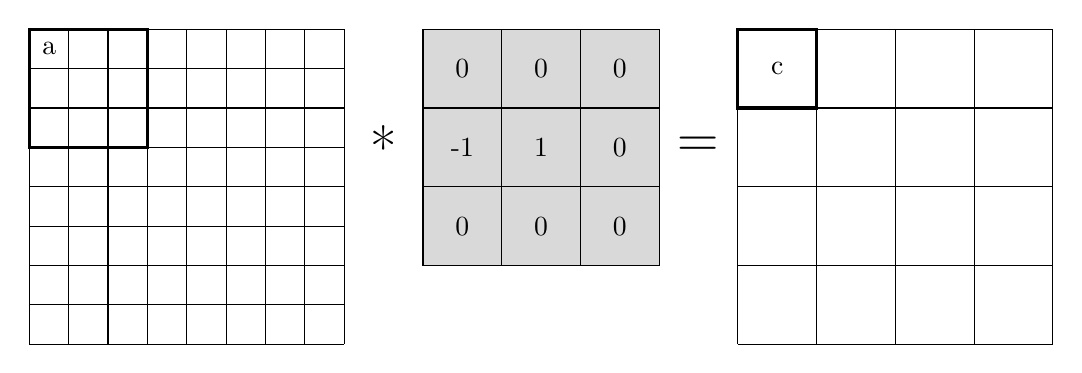
\begin{tikzpicture}
        \draw[step=0.5cm, black, thin](0,0) grid (4,4);
        \node (a_in) at (0.25, 3.75) {a};
        \filldraw[fill = gray!30, draw = black] (5,1) rectangle (8,4);
        \draw[step=1cm, black, thin](5,1) grid (8,4);
        \draw[step=0.5cm, black, line width=0.40mm](0,4) rectangle (1.5, 2.5);
        \node (ast) at (4.5, 2.5) {\huge *};
        \node at (5.5,3.5) {0};
        \node at (5.5,2.5) {-1};
        \node at (5.5,1.5) {0};
        \node at (6.5,3.5) {0};
        \node at (6.5,2.5) {1};
        \node at (6.5,1.5) {0};
        \node at (7.5,3.5) {0};
        \node at (7.5,2.5) {0};
        \node at (7.5,1.5) {0};
        \node (eq) at (8.5, 2.5) {\huge =};
        \draw[step=1cm, black, thin](9,0) grid (13,4);
        \filldraw[fill=white, draw=black, line width=0.40mm](9,4) rectangle (10,3);
        \node (c_out) at (9.5,3.5) {c};  
    \end{tikzpicture}
    \caption{Representación del proceso de obtención de la matriz convolucionada.}
\end{figure}

El filtro de convolución es la base del proceso de codificado de la imagen, la codificación se refiere a la transformación de una imagen a un vector de características de alta dimensión (\emph{downsampling}), una vez que se tiene el mapa de características sigue con el proceso de \emph{upsampling}.

\subsection{Modelo FPN}
La arquitectura de red neuronal tipo red piramidal de características, por sus siglas en inglés FPN\footnote{FPN: Feature Pyramid Network}, se trata de una estructura que funciona en conjunto con el codificador \texttt{ResNet}, mientras el codificador tiene la tarea de realizar el \emph{downsampling} de las dimensiones espaciales de la imágen de entrada y convertirlas a un mapa de característica , el decodificador hace justamente lo opuesto (\emph{up-sampling}), a partir del mapa de características producto de la codificación, realiza una secuencia de deconvoluciones que construyen la máscara de segmentación estimada.

\begin{figure}[H]
    \centering
    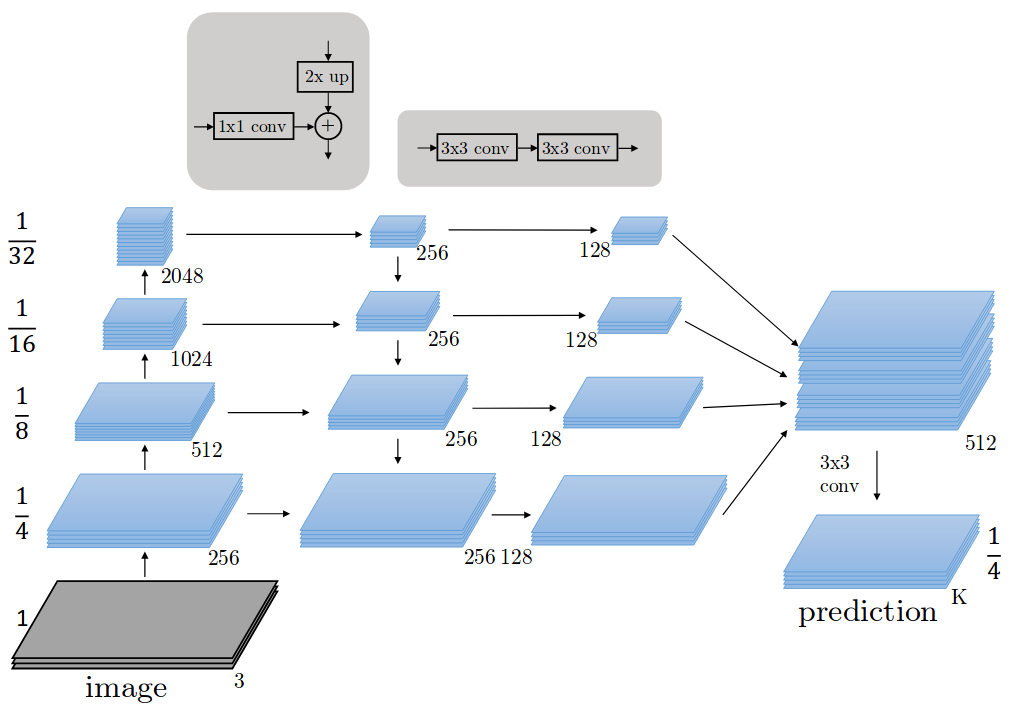
\includegraphics[scale=0.40]{Figuras/fpn_ar.png}
    \caption{Representación de la arquitectura FPN \citep{fpn_2}.}
    \label{fig:fpn_map}
\end{figure}
\coltext{Traducir etiquetas}

En la figura \ref{fig:fpn_map} se puede apreciar la arquitectura y la transformación de las dimensiones de los datos, el número a lado izquiero de las capas de convolución representa la resolución en proporción a la entrada y el número de lado derecho representa el número de canales. El número de canales aumenta mientras que la resolución disminuye.

\section{Implementación de la Solución}
Para la implementación de la herramienta propuesta, se utilizó \texttt{Python} como lenguaje principal. \texttt{Python} es un lenguaje de alto nivel con un extenso repositorio de paquetes desarrollados por la comunidad, también es un lenguaje ligero ideal para el procesamiento de datos y de operaciones con datos de altas dimensiones (\emph{high-dimensional data}), debído a esto último, se consideró \texttt{Python} la mejor opción para la implementación de la red neuronal profunda.

Si bien otros lenguajes tienen una mayor velocidad en la ejecución de cálculos complejos, es la facilidad con la que se pueden desplegar implementaciones complejas en relativamente pocas líneas de código lo que llevo a la conclusión de que \texttt{Python} es la opción ideal para la implementación propuesta, como el hecho de que existen muchas documentaciones e implementaciones similares en este lenguaje.

A continuación se especifican las librerías claves utilizadas para llevar a cabo la implementación, así mismo se da una breve descripción general sobre la misma y su importancia durante el desarollo de la propuesta.

\begin{table}[H]
    \centering
    \caption{Tabla de librerías utilizadas para la implementación de la propuesta.}
    \scalebox{0.90}{
    \begin{tabular}{|p{3cm}|p{10cm}|}
        \hline
        \bf{Librería} & \bf{Descripción} \\
        \hline
        \texttt{Torch.vision} & Este paquete es una colección de módulos relacionados con las operaciones de tensores y la aceleración de cálculos mediante hardware. Se usa en conjunto con \texttt{NumPY} y cuenta con las arquitecturas de redes neuronales típicas, así como herramientas para el cargado de datos y la configuración de parametros de los modelos.\\
        
        \hline
        \texttt{Quvel Segmentation Models} & Este paquete cuenta las arquitecturas de las redes neuronales de segmentación semántica típicas, se trata del marco de trabajo mediante el cuál podemos crear y configurar la arquitectura de la red para después realizar el entrenamiento.\\
        
        \hline
        \texttt{Numpy} & Esta librería fue desarrollada para habilitar el uso de vectores y matríces de grandes dimensiones y para la computación numérica en general, ya que \texttt{Python} originalmente no cuenta con el soporte para esto.\\
        
        \hline
        \texttt{OpenCV} & Es una librería dedicada al procesamiento de imágenes y a la visión computacional, cuenta con funciones que permiten cargar imágenes y obtener su matríz de pixeles así como aplicar efectos y transformaciones en estas.\\

        \hline
        \texttt{Albumentations} & Esta librería es principalmente útil para el pre-procesado de las imágenes al momento de realizar el entrenamiento, cuenta con funciones que permiten crear secuencias de transformaciones específicas para distíntos subconjuntos de datos así como la capacidad de transformar imágenes a tensores.\\

        \hline
    \end{tabular}}
    \label{tab:libs}
\end{table}

En el cuadro \ref{tab:specs} se especifícan las características del equipo en el cuál fue realizado el experimento.

\begin{table}[H]
    \centering
    \caption{Especificaciones técnicas de los componentes.}
    \begin{tabular}{|l|l|}
        \hline
        \bf{Componente} & \bf{Descripción} \\
        \hline
        Procesador & Ryzen 5 3600x, 3.80GHz, 6-Core \\
        \hline
        GPU & Nvidia GeForce 1050ti, 4gb \\
        \hline
        MOBO & Gigabyte Gaming AB-350 \\
        \hline
        RAM & HyperX Fury, 16gb, 2433mhz \\
        \hline
    \end{tabular}
    \label{tab:specs}
\end{table}
\subsection{Computación Asistída por Hardware}
Los cálculos llevados en el proceso de entrenamiento involucra realizar operaciones con datos de altas dimensiones (\emph{high-dimentional data}) los cuales requieren una gran cantidad de recursos de procesamiento, estas operaciones al estar relacionadas con vectores y matríces pueden ser ejecutadas rapidamente por la unidad GPU\footnote{GPU: Graphics Processor Unit}, entre mayor sea la velocidad de procesamiento de la GPU más rapido es el entrenamiento de nuevos modelos y con mayor resolución.

\subsection{Módulos de la Implementación}
La herramienta desarrollada en el presente trabajo de tesis se divide en cuatro módulos funcionales y un módulo central encargado de controlar la ejecución de los mismos. En la figura \ref{fig: modules} se puede observar la estrúctura modular del software desarrollad, dentro de dichos módulos se encuentran las funciones específicas de esa categoría y en el módulo principal se encuentran los parámetros del modelo.

\tikzstyle{block} = [rectangle, draw, fill=gray!20, 
    text width=7em, text centered, minimum height=4em]
\tikzstyle{line} = [draw, -latex']
\tikzstyle{cloud} = [draw, ellipse,fill=red!20, node distance=3cm,
    minimum height=2em]

\begin{figure}[H]
    \centering
    \begin{tikzpicture}[node distance = 1cm and 1cm]
        \node [block] (main) {main};
        \node [block, left= of main] (load) {load$\_$dataset};
        \node [block, right= of main] (train) {train$\_$model};
        \node [block, below= of main] (test) {test$\_$model};
        % Líneas
        \path [line] (load) -- (main);
        \path [line] (train) -- (main);
        \path [line] (test) -- (main);
    \end{tikzpicture}
    \caption{Distribución de los módulos en la herramienta desarrollada.}
    \label{fig: modules}
\end{figure}

\subsection{Cargado de Datos}
El proceso de cargado de datos y filtrado es un proceso muy importante para la ejecución correcta en las siguientes transformaciones, para el entrenamiento del modelo se utilizará una base de datos obtenida de la Asociación de Recolección de Imágenes dermatolólogicas, por sus siglas en inglés (\emph{ISIC}\footnote{ISIC: International Skin Imaging Collaboration.}). La base de datos de ISIC cuenta con 10mil imágenes de entrenamiento con resoluciones distintas, con diferentes tonos de iluminación y rotación, así como su máscara de segmentación conocida y 2mil imágenes para realizar pruebas, también con resoluciones no estandarizadas y sin máscara de segmentación.

\definecolor{folderbg}{RGB}{124,166,198}
\definecolor{folderborder}{RGB}{110,144,169}

\def\Size{4pt}
\tikzset{
  folder/.pic={
    \filldraw[draw=folderborder,top color=folderbg!50,bottom color=folderbg]
      (-1.05*\Size,0.2\Size+5pt) rectangle ++(.75*\Size,-0.2\Size-5pt);  
    \filldraw[draw=folderborder,top color=folderbg!50,bottom color=folderbg]
      (-1.15*\Size,-\Size) rectangle (1.15*\Size,\Size);
  }
}
\begin{figure}[H]
    \centering
    \begin{forest}
        for tree={
          font=\ttfamily,
          grow'=0,
          child anchor=west,
          parent anchor=south,
          anchor=west,
          calign=first,
          inner xsep=7pt,
          edge path={
            \noexpand\path [draw, \forestoption{edge}]
            (!u.south west) +(7.5pt,0) |- (.child anchor) pic {folder} \forestoption{edge label};
          },
          before typesetting nodes={
            if n=1
              {insert before={[,phantom]}}
              {}
          },
          fit=band,
          before computing xy={l=15pt},
        }  
      [Data
        [Train$\_$Images
        ]
        [Annot$\_$Images
        ]
        [Test$\_$Images
        ]
      ]
      \end{forest}
      \caption{Representación del árbol de directorios de imágenes.}    
\end{figure}


Lo primero que se desarrolló fue un asistente de cargado y filtrado de imágenes, en el código \ref{code:load} se puede apreciar el código fuente y las funciones utilizadas para tal motivo. Al ser utilizado el objeto \emph{dataset} y alimentar los argumentos con los directorios de las imágenes se obtiene como resultado un objeto de dimensión $n \times 2 \times (m \times n)$ donde $n$ es el número de muestras cargadas y el primer elemento de la fila es la matríz de la imágen real, y el segúndo la matríz de la máscara conocída.


\newcommand{\listingsfont}{\ttfamily}

\renewcommand{\lstlistingname}{Código}
\definecolor{codegreen}{rgb}{0,0.6,0}
\definecolor{codeblue}{rgb}{0.121, 0.203, 0.858}
\definecolor{codegray}{rgb}{0.5,0.5,0.5}
\definecolor{codepurple}{rgb}{0.58,0,0.82}
\definecolor{backcolour}{rgb}{0.95,0.95,0.92}

\lstdefinestyle{pystyle}{
    basicstyle=\linespread{1.5}\listingsfont,
    backgroundcolor=\color{backcolour},   
    commentstyle=\color{codegreen},
    keywordstyle=\color{codeblue},
    numberstyle=\tiny\color{codegray},
    stringstyle=\color{codepurple},
    basicstyle=\ttfamily\footnotesize,
    breakatwhitespace=false,         
    breaklines=true,                 
    captionpos=b,                    
    keepspaces=true,                 
    numbers=left,                    
    numbersep=5pt,                  
    showspaces=false,                
    showstringspaces=false,
    showtabs=false,                  
    tabsize=2
}
\lstset{style=pystyle}
\begin{lstlisting}[language = Python, label = {code:load} ,caption= Código fuente del asistente de cargado de imágenes.]
    # load_dataset.py
    # Creacion de la clase encargada de cargar, corregir y contener el conjunto de datos.

    class dataset ():
        def __init__(
            self,
            images_dir,
            masks_dir,
            classes=None,
        ):
        # Extraccion de ids de imagenes y mascaras.
        self.ids = listdir(images_dir)
        self.images_fps = [os.path.join(images_dir(img_id)
                          for img_id in self.ids]

        self.masks_fps = [os.path.join(mask_dir,
                         (img_id[:-4] + '_segmentation.png'))
                         for img_id in self.ids]

    # Lectura de imagenes y correcion de canales.
    def __getitem__(self,i):
        image = cv2.imread(self.images_fps[i])
        image = cv2.cvtColor(image, cv2.COLOR_BGR2RGB)

        mask = cv2.imread(self.masks_fps[i],0)

        return image, mask
\end{lstlisting}

A continuación se da un breve ejemplo del uso del asistente de cargado.

\begin{lstlisting}[language = Python, label = {code:load} ,caption= Uso de la clase.]

    # main.py.
    
    import load_dataset as ld 

    train_dir = 'Data/Train_Images'
    mask_dir = 'Data/Train_Images'

    set_de_datos = ld.dataset(train_dir, mask_dir)

    # Al ser un vector de matrices se puede obtener una muestra del conjunto de datos mediante su posicion indizada.

    imagen, mascara = set_de_datos[1]

    # Dando como resultado dos matrices.

\end{lstlisting}


\subsection{Pre-procesamiento}
El \emph{pre-procesamiento} se define como una secuencia de transformaciones que se aplican al momento previo del entrenamiento y afecta a un subconjunto específico de los datos. Para el diseño de la secuencia de transformaciones tanto para el subconjunto de entrenamiento como el subconjunto fueron consideradas las siguientes características.

\begin{description}
    \item[Resolución]{ El codifícador admite resoluciones específicas, debído a las dimensiones admitidas para el filtrado de convolución de matríces.}
    \item[Número de muestras]{La cantidad de datos disponibles para el entrenamiento afecta la precisión final, si el conjunto de datos es limitado se pueden realizar transformaciones de las imágenes presentes para obtener más datos de entrenamiento. Así como tener un conjunto muy extenso y con poca variabilidad afectaría también la capacidad de predecir imágenes generalizadas, se puede ajustar mediante el pre-procesamiento.}
    \item[] 
\end{description}


\tikzstyle{block} = [rectangle, draw, fill=gray!20, 
    text width=7.5em, text centered, minimum height=4em]
\tikzstyle{line} = [draw, -latex']
\tikzstyle{cloud} = [draw, ellipse,fill=red!20, node distance=3cm,
    minimum height=2em]

\begin{figure}[H]
    \centering
    \begin{tikzpicture}[node distance = 1cm and 1cm]
        \node [block] (input) {Imagen de Entrada ($m \times n$)};
        \node [block, below=of input, right= of input] (tr1) {Resize ($512 \times 512$)};
        \node [block, right= of tr1] (tr2) {Interpolate (INTER$\_$AREA)};
        \node [block, right= of tr2] (tr3) {Transpose (2, 0, 1)};
        \node [block, below= of tr3] (out) {Dato de Salida ($N \times (512 \times 512)$)};
        % Líneas
        \path [line] (input) -- (tr1);
        \path [line] (tr1) -- (tr2);
        \path [line] (tr2) -- (tr3);
        \path [line] (tr3) -- (out);

    \end{tikzpicture}
    \caption{Línea de pre-procesado.}
    \label{fig: pipeline}
\end{figure}

Debido a que el \emph{dataset} es extenso y solo clasifíca entre dos categorías, no es necesario realizar demasiadas trasnformaciones, no obstante es importante trasponer la matríz de entrada para convertir la matríz a tensor.

\subsection{Entrenamiento y Validación}
Para poder determinar la eficiencia durante el \emph{entrenamiento} y optimizar los pesos sinápticos es necesario hacer uso de métricas, dichas métricas se aplicarán sobre el subconjunto de validación. Los datos utilizados fueron divididos en una proporción de $70\%$ para entrenamiento y $30\%$ para la validación, el subconjunto de validación no es usado durante el entrenamiento, sino qué, al terminar una época se verifíca con ese subconjunto la precisión.


La métrica utilizada para evaluar el modelo es la del \emph{índice de Jaccard} (\emph{Intersection Over Union}) por sus siglas en inglés (IoU) \citep{fpn_1} de la siguiente ecuación,

\begin{equation}\label{eq:jacc}
    J(A,B) = \frac{|A \cap B|}{| A \cup B |} = \frac{|A \cap B|}{|A| + |B| - |A \cap B|}
\end{equation} 

donde $A$ y $B$ se pueden interpretar como la máscara real y la máscara estimada, y debido a que las imágenes consisten de pixeles, la ecuación anterior se puede representar en el caso de objetos discretos como

\begin{equation}
    J = \frac{1}{n} \sum_{c=1}^{k} W_c \sum_{i=1}^{n}\frac{y_i^c \hat y_i^c}{y_i^c + \hat y_i^c - y_i^c \hat y_i^c}
\end{equation} 

donde $y_i^c$ y $\hat y_i^c$ son valores binarios y corresponden a la probabilidad de que el pixel $i$ corresponda a la clase $c$ de un número $k$ de clases.

Mediante la librería de Yakubovskiy \citep{Yakubovskiy:2019}, se pueden configurar los parámetros previamente al entrenamiento.

\begin{lstlisting}[language = Python, label = {code:load} ,caption= Ejemplo de configuración de parámetros. ]
    # main.py.
    import segmentation_models_pytorch as smp 

    metrics = [smp.utils.metrics.IoU(threshold=0.5),]
    loss = smp.utils.losses.DiceLoss()
    optimizer = torch.optim.Adam([dict(params=model.parameters(), lr= 0.0001),])
\end{lstlisting}

\subsection{Predicción de Máscaras} 
Una vez obtenido un modelo con precisión buena (\emph{good fit}), el objetivo es generar máscaras desconocidas a partír de las imágenes del set de pruebas. Para esto es necesario popular de nuevo un \emph{dataset} de dimensión $N \times (m \times n)$, básicamente es un vector de matríces donde $N$ es el número de imágenes para realizar la prueba, y $m \times n$ es la resolución de imágen de la cuál se desea obtener la máscara de segmentación.

\chapter{Experimentos}
En este capítulo se presentan los experimentos llevados a cabo durante el desarrollo de la herramienta propuesta. Las siguientes secciones corresponden a diferentes experimentos llevados a cabo para validar la hipótesis del presente trabajo de tesis, cada experimento contiene tres subsecciones: \emph{diseño experimental}, \emph{resultados} y \emph{discusión}.

En la subsección de \emph{diseño experimental}, se detalla el experimento y el parámetro que se pretende definir en base a este, todos los procesos realizados por la herramienta desarrollada en el presente trabajo de tesis se ejecutan de forma secuencial, debido a esto es necesario determinar el mejor parámetro en cada paso de la transformación.

En \emph{resultados}, se reporta e interpreta todos los resultados obtenidos mediante el experimento llevado a cabo en esa sección, cada experimento cuenta con su propia sección y se determina el mejor parámetro para realizar el experimento siguiente. 

Y para finalizar en \emph{discusión}, se llega una conclusión basandose en los resultados obtenidos y la información que representan las gráficas.


\section{Estadísticas de los Datos de Entrada} 
Este experimento tiene como objetivo determinar el codificador ideal para la arquitectura implementada basandosé en la información estadística del conjunto de datos de las imágenes, también determinar las transformaciones necesarias para coincidir con las dimensiones requeridas por la arquitectura y las ofrecidas por la imagen.

\subsection{Diseño Experimental}
Las métricas que serán evaluadas del conjunto de datos de entrenamiento son las siguientes:
\begin{description}
    \item[Muestras] El número de muestras del conjunto de datos puede determinar las transformaciones posteriores tanto para reducir \emph{overfit} como para mejorar el \emph{underfit}.
    \item[Clases] La cantidad de clases entre las que el modelo tiene que clasificar determina la complejidad computacional de éste, por lo tanto también determina transformaciones requeridas.
    \item[]  
\end{description}
\subsection{Resultados}
\subsection{Discusión}

\section{Evaluación del Aprendizaje}
Una vez seleccionado el codificador ideal, es necesario evaluar la configuración del modelo en la época presente y configuración actual, al finalizar cada ciclo de entrenamiento se realiza una validación con el porcentaje del conjunto de datos que no fue utilizado durante éste.
\subsection{Diseño Experimental}
Para determinar un valor probabilistico entre dos mapas de valores binarios es necesario utilizar un coeficiente que evalúe la similitud entre ambos conjuntos de datos, siendo el conjunto $A$ la máscara real o \emph{ground truth}, y el conjunto $B$ el mapa obtenido por la computación del modelo se utilizó el criterio de dados para determinar la probabilidad ($0 \% - 100 \%$), la ecuación del criterio de dados dice que la probabilidad de que dos mapas binarios sean iguales es dos veces la cantidad de pixeles sobrepuestos o idénticos entre la suma de los pixeles de ambos mapas, 

\begin{equation}\label{eq:diceloss}
    \text{DC} = \frac{2|A \cap B |}{|A| + |B|}
\end{equation}

donde $A$ es un mapa binario de pixeles que representa la máscara real y $B$ la máscara de segmentación obtenida por el modelo.

\def\firstcircle{(0,0) circle (1.5cm)}
\def\secondcircle{(2,0) circle (1.5cm)}
\def\thirdcircle{(0:2cm) circle (1.5cm)}

\begin{figure}[b]
    \centering
    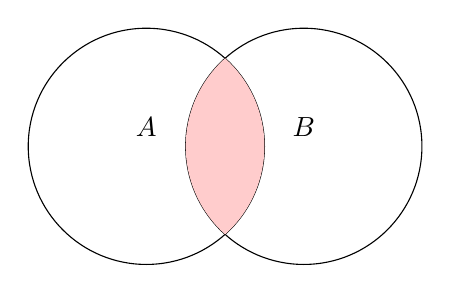
\begin{tikzpicture}
        \draw \firstcircle node [above] {$A$};
        \draw \secondcircle node [above] {$B$};
        %\node at (-2, 0) {\large $2 \times$};
        \begin{scope}
            \clip \firstcircle;
            \fill[red!20] \secondcircle;
        \end{scope}
    \end{tikzpicture}
    \caption{Representación de la región de sobreposición de pixeles en el coeficiente de dados.}
\end{figure}

\subsection{Resultados}
\subsection{Discusión}

\section{Criterio de Jaccard}
En la sección anterior, el criterio de dados es utilizado para evaluar la similitud entre un mapa binario y un mapa probabilistico correspondiente a la máscara conocida y la máscara estimada, durante el entrenamiento del modelo. Sin embargo para validar el resultado final es necesario utilizar una métrica similar, que penalice más el error o la diferencia entre ambos mapas.

\subsection{Diseño Experimental}
Para determinar un porcentaje de similitud entre la máscara estimada con la máscara conocida o también denominada verdad absoluta (\emph{ground truth}) podemos utilizar una métrica como la de la ecuación \ref{eq:jacc}, el índice de Jaccard. Este criterio es relativamente similar al coeficiente de dados de la ecuación \ref{eq:diceloss}, mediante el solapado de ambas máscaras se promedía la coincidencia entre pixeles, sin embargo en el criterio \emph{IoU} el error tiene mayor penalización, por lo que se podría decir que es una versión mas robusta de evaluación ideal para evaluar el modelo final.

\def\rectA{(0,0) rectangle (2,2)}
\def\rectB{(3,-1) rectangle (1,1)}

\begin{figure}[b]
    \centering
    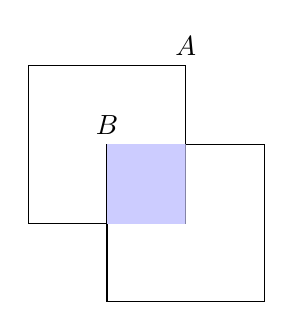
\begin{tikzpicture}
        \draw \rectA node [above] {$A$};
        \draw \rectB node [above] {$B$};
        %\node at (-2, 0) {\large $2 \times$};
        \begin{scope}
            \clip \rectA;
            \fill[blue!20] \rectB;
        \end{scope}
    \end{tikzpicture}
    \caption{Representación de la región de sobreposición de pixeles en el índice de Jaccard.}
\end{figure}


\subsection{Resultados}
\subsection{Discusión}


\chapter{Conclusiones}
\section{Discusión}

\section{Trabajo a Futuro}

\nocite{*}